\documentclass[11pt]{article}
\usepackage[margin=0.7in]{geometry}
\usepackage{booktabs}
\usepackage{amsmath,amssymb}
\usepackage{xcolor}
\usepackage{tikz}
\usetikzlibrary{arrows.meta,positioning,shapes.geometric,fit,backgrounds}
\definecolor{loopblue}{RGB}{37,99,235}
\definecolor{loopred}{RGB}{220,38,38}
\definecolor{loopgreen}{RGB}{22,163,74}
\definecolor{looporange}{RGB}{234,88,12}
\definecolor{looppurple}{RGB}{124,58,237}
\definecolor{loopgreenDark}{RGB}{21,128,61}

\begin{document}
\pagestyle{empty}
\begin{center}
{\LARGE Figure Gallery}\\[2pt]
{\small 10 figures for \textit{The Dynamic Reflexive Loop and the Five Organs}. Pick by number (e.g., ``1, 3, 5, 7, 9'') and I will wire them into \texttt{main.tex}.}
\end{center}
\vspace{8pt}

% --- FIGURE 1: The One Loop ---
\begin{center}
\textbf{Figure 1 — The One Loop (System $\leftrightarrow$ World, two channels)}
\end{center}
\begin{center}
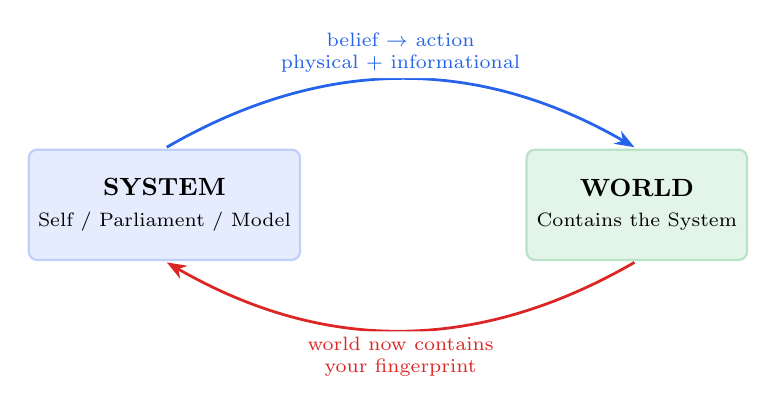
\begin{tikzpicture}[thick]
  \node[draw, rounded corners=3pt, fill=loopblue!12, draw=loopblue!30, minimum width=2.8cm, minimum height=1.4cm, align=center, font=\small] (sys) at (0,0) {\textbf{SYSTEM}\\\scriptsize Self / Parliament / Model};
  \node[draw, rounded corners=3pt, fill=loopgreen!12, draw=loopgreen!30, minimum width=2.8cm, minimum height=1.4cm, align=center, font=\small] (world) at (6,0) {\textbf{WORLD}\\\scriptsize Contains the System};
  \draw[-{Stealth[length=2.5mm]}, loopblue, line width=1.0pt, shorten >=1pt, shorten <=1pt] (sys.north) to[out=30,in=150] node[midway, above, font=\scriptsize, fill=white, inner sep=2pt, rounded corners=1pt, align=center] {belief $\to$ action\\physical + informational} (world.north);
  \draw[-{Stealth[length=2.5mm]}, loopred, line width=1.0pt, shorten >=1pt, shorten <=1pt] (world.south) to[out=-150,in=-30] node[midway, below, font=\scriptsize, fill=white, inner sep=2pt, rounded corners=1pt, align=center] {world now contains\\your fingerprint} (sys.south);
\end{tikzpicture}
\end{center}
{\scriptsize \textbf{Use:} Introduction or \S Loop. Two channels, three consequences (models rot, measurement corrupts, truth moves).}

\vspace{14pt}
% --- FIGURE 2: Expanding Loop ---
\begin{center}
\textbf{Figure 2 — The Expanding Reflexive Loop}
\end{center}
\begin{center}
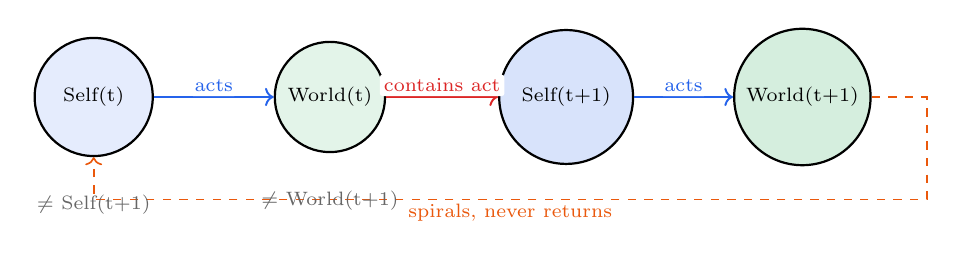
\begin{tikzpicture}[thick, every node/.style={font=\scriptsize}]
  \node[draw, circle, fill=loopblue!12, minimum size=1.5cm, align=center] (s0) at (0,0) {Self(t)};
  \node[draw, circle, fill=loopgreen!12, minimum size=1.4cm, align=center] (w0) at (3,0) {World(t)};
  \node[draw, circle, fill=loopblue!18, minimum size=1.7cm, align=center] (s1) at (6,0) {Self(t+1)};
  \node[draw, circle, fill=loopgreen!18, minimum size=1.5cm, align=center] (w1) at (9,0) {World(t+1)};
  \draw[->, loopblue, line width=0.7pt] (s0) -- node[above, font=\scriptsize, fill=white, inner sep=1.5pt, rounded corners=1pt] {acts} (w0);
  \draw[->, loopred, line width=0.7pt] (w0) -- node[above, font=\scriptsize, fill=white, inner sep=1.5pt, rounded corners=1pt] {contains act} (s1);
  \draw[->, loopblue, line width=0.7pt] (s1) -- node[above, font=\scriptsize, fill=white, inner sep=1.5pt, rounded corners=1pt] {acts} (w1);
  \draw[->, looporange, line width=0.6pt, dashed] (w1.east) -- ++(0.7,0) -- ++(0,-1.3) -| (s0.south) node[pos=0.25, below, font=\scriptsize, fill=white, inner sep=1.5pt, rounded corners=1pt] {spirals, never returns};
  \node[below=0.35cm of s0, font=\scriptsize, text=black!60] {$\neq$ Self(t+1)};
  \node[below=0.35cm of w0, font=\scriptsize, text=black!60] {$\neq$ World(t+1)};
\end{tikzpicture}
\end{center}
{\scriptsize \textbf{Use:} \S Expanding loop. Self(t+1) $\neq$ Self(t), World(t+1) $\neq$ World(t), spirals wider.}

\vspace{14pt}
% --- FIGURE 3: Five Organs Cycle ---
\begin{center}
\textbf{Figure 3 — The Five Organs as a Cycle}
\end{center}
\begin{center}
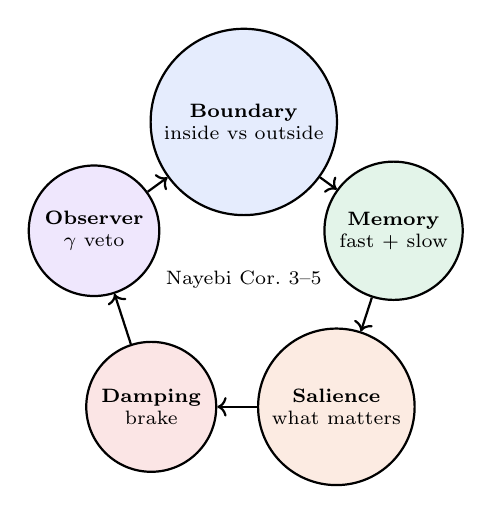
\begin{tikzpicture}[thick]
  \def \r{2.0cm}
  \node[draw, circle, fill=loopblue!12, minimum size=1.50cm, align=center, font=\scriptsize] (b) at (90:\r) {\textbf{Boundary}\\\scriptsize inside vs outside};
  \node[draw, circle, fill=loopgreen!12, minimum size=1.50cm, align=center, font=\scriptsize] (m) at (18:\r) {\textbf{Memory}\\\scriptsize fast + slow};
  \node[draw, circle, fill=looporange!12, minimum size=1.50cm, align=center, font=\scriptsize] (s) at (-54:\r) {\textbf{Salience}\\\scriptsize what matters};
  \node[draw, circle, fill=loopred!12, minimum size=1.50cm, align=center, font=\scriptsize] (d) at (-126:\r) {\textbf{Damping}\\\scriptsize brake};
  \node[draw, circle, fill=looppurple!12, minimum size=1.50cm, align=center, font=\scriptsize] (o) at (162:\r) {\textbf{Observer}\\\scriptsize $\gamma$ veto};
  \draw[->, thick] (b) -- (m); \draw[->, thick] (m) -- (s); \draw[->, thick] (s) -- (d); \draw[->, thick] (d) -- (o); \draw[->, thick] (o) -- (b);
  \node[font=\scriptsize] at (0,0) {Nayebi Cor.\ 3--5};
\end{tikzpicture}
\end{center}
{\scriptsize \textbf{Use:} Introduction or \S Five Organs. The warp — lose one and a task distribution exploits the gap.}

\vspace{14pt}
% --- FIGURE 4: Five Organs at Every Scale (table) ---
\begin{center}
\textbf{Figure 4 — Five Organs at Every Scale}
\end{center}
{\scriptsize
\begin{center}
\begin{tabular}{p{1.9cm}p{2.0cm}p{2.0cm}p{2.2cm}p{2.0cm}p{2.4cm}}
\toprule
Scale & Boundary & Memory & Salience & Damping & Observer \\
\midrule
Molecule & Lipid membrane & E-LTP / L-LTP & Ca$^{2+}$+DA/NE & LTD/BCM & BCM $\theta_m$ \\
Mind & Narrative self & Hippo / cortex & Affect [0.5,2.0] & PFC veto & $\gamma$-gate \\
Harness & Ledger & Light $\to$ Deep & AffectState & cull\_failed & $\gamma$-gate \\
Universe & Horizon & Measure / law & Inflation & Expansion & Awareness \\
\bottomrule
\end{tabular}
\end{center}
}
{\scriptsize \textbf{Use:} \S Five Organs or \S Levels. Same five, different substrate. Full 8-row table in paper.}

\vspace{14pt}
% --- FIGURE 5: Nested Levels ---
\begin{center}
\textbf{Figure 5 — How the Eight Levels Nest}
\end{center}
\begin{center}
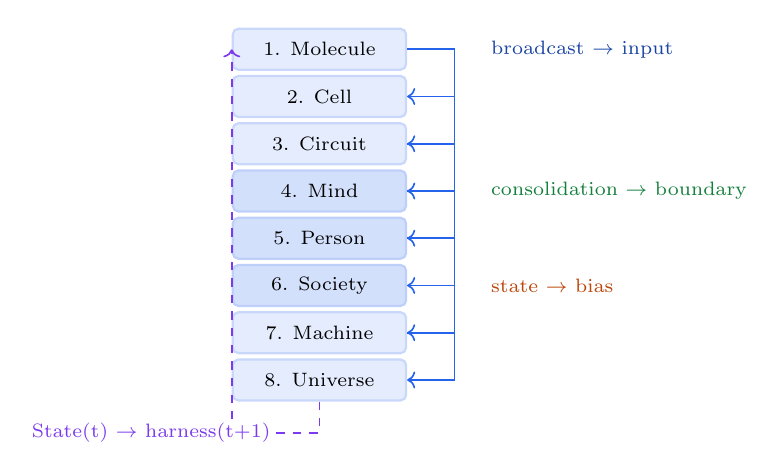
\begin{tikzpicture}[thick, every node/.style={font=\scriptsize}]
  \node[draw, rounded corners=2pt, fill=loopblue!12, draw=loopblue!25, minimum width=2.2cm, minimum height=0.52cm, align=center] (l1) at (0,3.6) {1. Molecule};
  \node[draw, rounded corners=2pt, fill=loopblue!12, draw=loopblue!25, minimum width=2.2cm, minimum height=0.52cm, align=center] (l2) at (0,3.0) {2. Cell};
  \node[draw, rounded corners=2pt, fill=loopblue!12, draw=loopblue!25, minimum width=2.2cm, minimum height=0.52cm, align=center] (l3) at (0,2.4) {3. Circuit};
  \node[draw, rounded corners=2pt, fill=loopblue!20, draw=loopblue!30, minimum width=2.2cm, minimum height=0.52cm, align=center] (l4) at (0,1.8) {4. Mind};
  \node[draw, rounded corners=2pt, fill=loopblue!20, draw=loopblue!30, minimum width=2.2cm, minimum height=0.52cm, align=center] (l5) at (0,1.2) {5. Person};
  \node[draw, rounded corners=2pt, fill=loopblue!20, draw=loopblue!30, minimum width=2.2cm, minimum height=0.52cm, align=center] (l6) at (0,0.6) {6. Society};
  \node[draw, rounded corners=2pt, fill=loopblue!12, draw=loopblue!25, minimum width=2.2cm, minimum height=0.52cm, align=center] (l7) at (0,0.0) {7. Machine};
  \node[draw, rounded corners=2pt, fill=loopblue!12, draw=loopblue!25, minimum width=2.2cm, minimum height=0.52cm, align=center] (l8) at (0,-0.6) {8. Universe};
  \foreach \i in {1,...,7} {
    \pgfmathtruncatemacro{\j}{\i+1}
    \draw[->, loopblue, line width=0.6pt] (l\i.east) -- ++(0.6,0) |- (l\j.east);
  }
  \node[right=1.0cm of l1, font=\scriptsize, text=loopblue!70!black, fill=white, inner sep=1.5pt, rounded corners=1pt, align=left] {broadcast $\to$ input};
  \node[right=1.0cm of l4, font=\scriptsize, text=loopgreenDark, fill=white, inner sep=1.5pt, rounded corners=1pt, align=left] {consolidation $\to$ boundary};
  \node[right=1.0cm of l6, font=\scriptsize, text=looporange!80!black, fill=white, inner sep=1.5pt, rounded corners=1pt, align=left] {state $\to$ bias};
  \draw[->, looppurple, line width=0.6pt, dashed] (l8.south) -- ++(0,-0.4) -| (l1.west) node[pos=0.25, left, font=\scriptsize, fill=white, inner sep=1.5pt, rounded corners=1pt] {State(t) $\to$ harness(t+1)};
\end{tikzpicture}
\end{center}
{\scriptsize \textbf{Use:} \S How it all works at every level. One loop nested 8 times — broadcast $\to$ input, consolidation $\to$ boundary, state $\to$ bias.}

\vspace{14pt}
% --- FIGURE 6: Parliament ---
\begin{center}
\textbf{Figure 6 — The Parliament (coalition competition $\to$ winner broadcast)}
\end{center}
\begin{center}
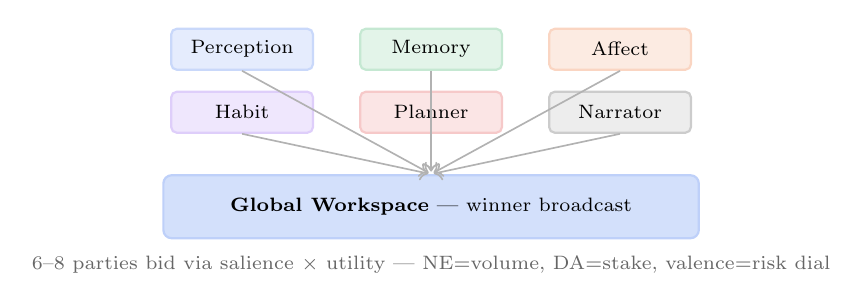
\begin{tikzpicture}[thick, every node/.style={font=\scriptsize}]
  \node[draw, rounded corners=2pt, fill=loopblue!12, draw=loopblue!25, minimum width=1.8cm, minimum height=0.52cm, align=center] (p) at (-2.4,1.3) {Perception};
  \node[draw, rounded corners=2pt, fill=loopgreen!12, draw=loopgreen!25, minimum width=1.8cm, minimum height=0.52cm, align=center] (m) at (0,1.3) {Memory};
  \node[draw, rounded corners=2pt, fill=looporange!12, draw=looporange!25, minimum width=1.8cm, minimum height=0.52cm, align=center] (a) at (2.4,1.3) {Affect};
  \node[draw, rounded corners=2pt, fill=looppurple!12, draw=looppurple!25, minimum width=1.8cm, minimum height=0.52cm, align=center] (h) at (-2.4,0.5) {Habit};
  \node[draw, rounded corners=2pt, fill=loopred!12, draw=loopred!25, minimum width=1.8cm, minimum height=0.52cm, align=center] (pl) at (0,0.5) {Planner};
  \node[draw, rounded corners=2pt, fill=gray!14, draw=gray!40, minimum width=1.8cm, minimum height=0.52cm, align=center] (n) at (2.4,0.5) {Narrator};
  \node[draw, rounded corners=3pt, fill=loopblue!20, draw=loopblue!30, minimum width=6.8cm, minimum height=0.80cm, align=center] (ws) at (0,-0.7) {\textbf{Global Workspace} — winner broadcast};
  \foreach \src in {p,m,a,h,pl,n} \draw[->, gray!60, line width=0.6pt, shorten >=1pt] (\src.south) -- (ws.north);
  \node[below=0.15cm of ws, font=\scriptsize, text=black!60, align=center, fill=white, inner sep=1.5pt, rounded corners=1pt] {6--8 parties bid via salience $\times$ utility — NE=volume, DA=stake, valence=risk dial};
\end{tikzpicture}
\end{center}
{\scriptsize \textbf{Use:} \S Mind or \S Parliament. No captain, configuration votes, winner experienced as ``my thought'' 200ms after.}

\vspace{14pt}
% --- FIGURE 7: Gamma-Gate ---
\begin{center}
\textbf{Figure 7 — The $\gamma$-Gate (slower loop vetoing faster one)}
\end{center}
\begin{center}
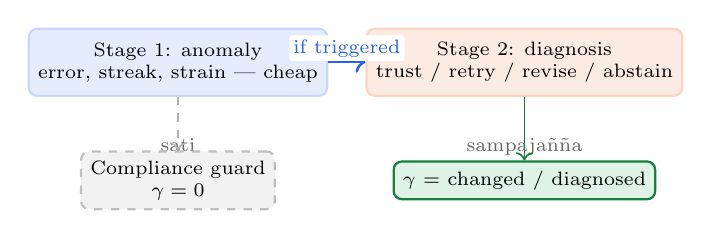
\begin{tikzpicture}[thick, every node/.style={font=\scriptsize}]
  \node[draw, rounded corners=3pt, fill=loopblue!12, draw=loopblue!25, minimum width=3.0cm, minimum height=0.85cm, align=center] (s1) at (-2.2,0) {Stage 1: anomaly\\{\scriptsize error, streak, strain — cheap}};
  \node[draw, rounded corners=3pt, fill=looporange!12, draw=looporange!25, minimum width=3.0cm, minimum height=0.85cm, align=center] (s2) at (2.2,0) {Stage 2: diagnosis\\{\scriptsize trust / retry / revise / abstain}};
  \draw[->, loopblue, line width=0.9pt] (s1) -- node[above, font=\scriptsize, fill=white, inner sep=1.5pt, rounded corners=1pt] {if triggered} (s2);
  \node[below=0.4cm of s1, font=\scriptsize, text=black!60, align=center] {sati};
  \node[below=0.4cm of s2, font=\scriptsize, text=black!60, align=center] {sampaja\~n\~na};
  \node[draw, rounded corners=3pt, fill=loopgreen!14, draw=loopgreenDark, minimum width=2.0cm, align=center] (g) at (2.2,-1.5) {$\gamma$ = changed / diagnosed};
  \draw[->, loopgreenDark, line width=0.6pt] (s2.south) -- (g.north);
  \node[draw, dashed, rounded corners=3pt, fill=gray!10, draw=gray!50, minimum width=2.0cm, align=center] (cg) at (-2.2,-1.5) {Compliance guard\\{\scriptsize $\gamma=0$}};
  \draw[->, gray!60, line width=0.6pt, dashed] (s1.south) -- (cg.north);
\end{tikzpicture}
\end{center}
{\scriptsize \textbf{Use:} \S Observer. Why $\gamma$ not accuracy — accuracy can be gamed by always saying ``no.''}

\vspace{14pt}
% --- FIGURE 8: Three Sides ---
\begin{center}
\textbf{Figure 8 — Reality, Perception, and Self as One Loop's Three Sides}
\end{center}
\begin{center}
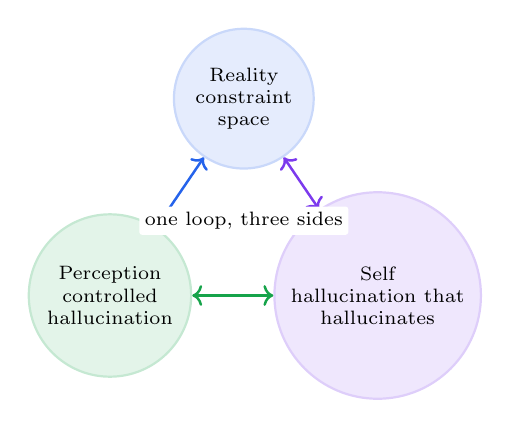
\begin{tikzpicture}[thick, every node/.style={font=\scriptsize}]
  \node[draw, circle, fill=loopblue!12, draw=loopblue!25, minimum size=1.75cm, align=center] (r) at (0,1.6) {Reality\\{\scriptsize constraint}\\{\scriptsize space}};
  \node[draw, circle, fill=loopgreen!12, draw=loopgreen!25, minimum size=1.75cm, align=center] (p) at (-1.7,-0.9) {Perception\\{\scriptsize controlled}\\{\scriptsize hallucination}};
  \node[draw, circle, fill=looppurple!12, draw=looppurple!25, minimum size=1.75cm, align=center] (s) at (1.7,-0.9) {Self\\{\scriptsize hallucination that}\\{\scriptsize hallucinates}};
  \draw[<->, loopblue, line width=0.9pt] (r) -- (p);
  \draw[<->, loopgreen, line width=0.9pt] (p) -- (s);
  \draw[<->, looppurple, line width=0.9pt] (s) -- (r);
  \node[font=\scriptsize, fill=white, inner sep=2pt, rounded corners=1pt] at (0,0.05) {one loop, three sides};
\end{tikzpicture}
\end{center}
{\scriptsize \textbf{Use:} \S Reality/Perception/Self. All three are controlled hallucinations, maintained not found.}

\vspace{14pt}
% --- FIGURE 9: Four Methods ---
\begin{center}
\textbf{Figure 9 — Four Methods, One Destination}
\end{center}
{\scriptsize
\begin{center}
\begin{tabular}{p{2.5cm}p{2.6cm}p{2.8cm}p{3.0cm}}
\toprule
Method & Substrate & Instrument & Shares with others \\
\midrule
Evolution & Worm, 302 & Natural selection & Nothing — except constraint \\
Connectomics & Fly, 140k & Electron microscopy & Nothing — except constraint \\
Mathematics & Theorem, 23pp & Selection, regret & Nothing — except constraint \\
Engineering & Harness, 11 mod & Code, audit trail & Nothing — except constraint \\
\midrule
\multicolumn{4}{c}{\textit{Only the constraint. That's why convergence is informative.}} \\
\bottomrule
\end{tabular}
\end{center}
}
{\scriptsize \textbf{Use:} Introduction or \S What it all means. Four methods share nothing except the constraint.}

\vspace{14pt}
% --- FIGURE 10: Only Real Choice ---
\begin{center}
\textbf{Figure 10 — The Only Real Choice}
\end{center}
\begin{center}
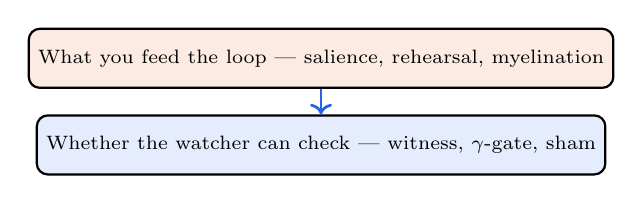
\begin{tikzpicture}[thick, every node/.style={font=\scriptsize}]
  \node[draw, rounded corners, fill=looporange!12, minimum width=5.2cm, minimum height=0.75cm, align=center] (a) {What you feed the loop — salience, rehearsal, myelination};
  \node[draw, rounded corners, fill=loopblue!12, minimum width=5.2cm, minimum height=0.75cm, align=center] (b) at (0,-1.1) {Whether the watcher can check — witness, $\gamma$-gate, sham};
  \draw[->, loopblue, line width=1pt] (a.south) -- (b.north);
\end{tikzpicture}
\begin{center}
\scriptsize
\begin{tabular}{p{5.8cm}p{5.8cm}}
\toprule
Pick what you rehearse & Externalize the witness — write \\
Protect sleep & Never let a fast loop grade its own homework \\
Buy BDNF & You don't choose whether to feed the loop \\
& \quad — only what you feed it \\
\bottomrule
\end{tabular}
\end{center}
\end{center}
{\scriptsize \textbf{Use:} \S Only Real Choice or Conclusion. The two things that are choosable.}

\vspace{8pt}
\hrule
\vspace{6pt}
\begin{center}
{\small Pick by number (e.g., ``1, 3, 5, 7, 9'') and the chosen ones will be wired into \texttt{main.tex} at the right sections. All figures are TikZ — no external files, compile with \texttt{pdflatex}.}
\end{center}

\end{document}
